\section{Le site de l'OFNI}
\sectitle{Le site internet de l'OFNI}

\begin{frame}
    \frametitle{Introduction}
    \centering
    \textbf{Objectif}: Concevoir et développer un nouveau site web pour l’\ofni
    \vspace{1,2cm}

    \pause

    \textbf{Processus}: 
    \begin{itemize}
        \item Analyse des besoins
        \item Maquettage
        \item Choix des technologies
        \item Implémentation des différentes fonctionnalités
    \end{itemize}
\end{frame}

\begin{frame}
    \frametitle{Le site web de l’association OFNI}
    % \centering

    \begin{columns}
    \column{0.5\textwidth}
    \textbf{Trois phases :}
    \bigskip

    \begin{enumerate}
        \item Maquettage du site
        \item Développement du site
        \item Réalisation du rapport et de la soutenance orale
    \end{enumerate}
    \column{0.5\textwidth}
    \centering
    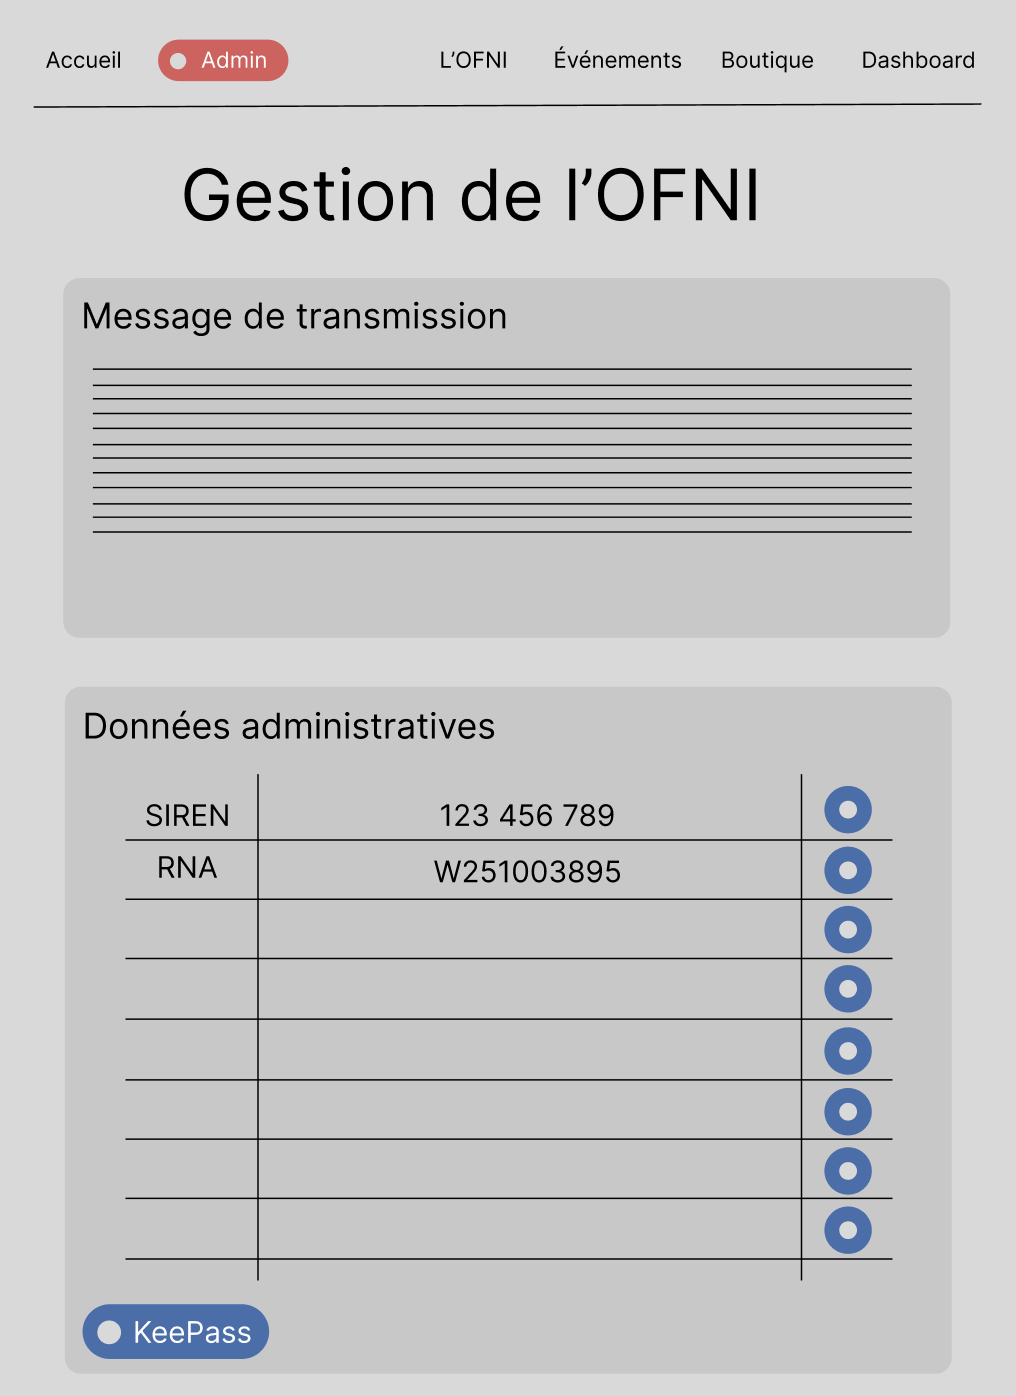
\includegraphics[height=1.2\textwidth]{pictures/figma.png}
    \end{columns}
\end{frame}

\begin{frame}
    \frametitle{Le site web de l’association OFNI}
    \centering
    \vspace{0.4cm}
    \ofni : Association des étudiants en informatique de l’Université
    \vspace{0.7cm}

    \pause
    
    \textbf{Pourquoi ce projet?} Ancien site obsolète, non mis à jour, pas de version mobile, ne répond plus aux besoins actuels
    \vspace{0.4cm}

    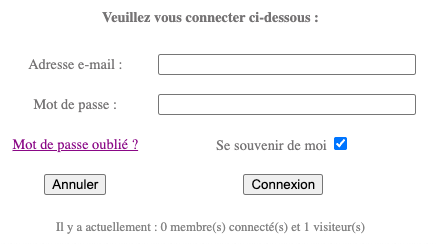
\includegraphics[height=0.35\textwidth]{pictures/img-old-site.png}
\end{frame}
